\chapter{Resultados}

Nesta seção, apresentamos os principais resultados positivos obtidos com a aplicação desenvolvida para análise do crescimento de plantas via processamento de imagens.

\section{Resultados do Algoritmo}

A aplicação do algoritmo de segmentação proposto resultou em máscaras precisas para a identificação das regiões vegetais nas imagens analisadas, mesmo diante de desafios como variações de iluminação, ruído de fundo e diferenças morfológicas entre as plantas. Os resultados evidenciam que o método é capaz de isolar de forma consistente as áreas verdes, minimizando a inclusão de regiões não pertencentes à planta e preenchendo eventuais falhas na segmentação.

As medidas morfológicas extraídas --- altura, largura e área foliar --- apresentaram boa estabilidade e reprodutibilidade ao longo de diferentes imagens e coleções, permitindo o acompanhamento quantitativo do crescimento das plantas. A sobreposição visual das máscaras segmentadas e das linhas de medição sobre as imagens originais facilita a validação dos resultados, tornando o processo transparente e confiável para o usuário.

\section{Acompanhamento do Crescimento de uma Planta}

A interface gráfica proporciona uma experiência intuitiva e eficiente para o usuário. Por meio dela, é possível organizar fotos em coleções, processar imagens individualmente ou em lote, visualizar resultados detalhados e acompanhar o desenvolvimento das plantas ao longo do tempo. A Figura~\ref{fig:interface-grafica} ilustra a tela principal da aplicação, destacando a organização das coleções.

\begin{figure}[H]
    \centering
    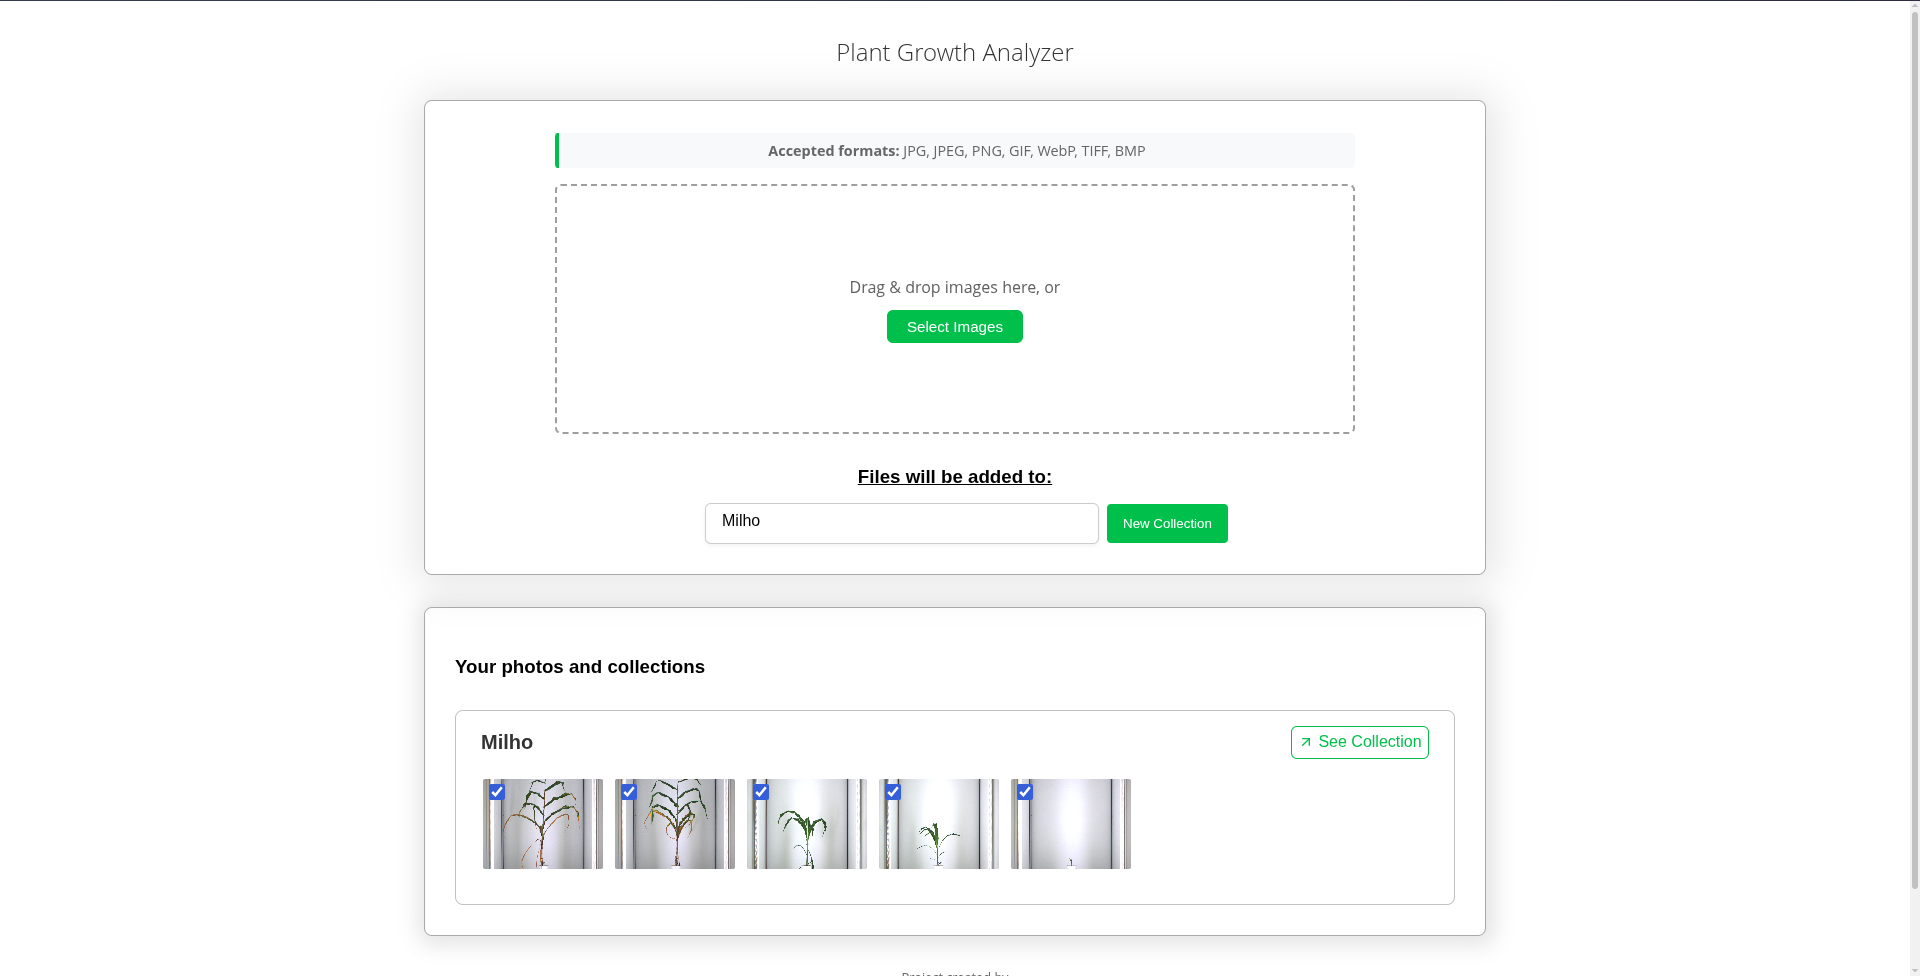
\includegraphics[width=0.9\textwidth]{../figures/screens/interface-grafica.png}
    \caption{Interface gráfica da aplicação. Na imagem, temos a tela inicial do aplicativo, com a opção de enviar imagens para a aplicação. Fonte: os autores.}
    \label{fig:interface-grafica}
\end{figure}

A interface gráfica pode ser dividida em três principais modos de visualização, cada um voltado para uma etapa do fluxo de trabalho do usuário:

\textbf{1. Visualização de Coleções:} A tela inicial da aplicação apresenta as coleções de imagens organizadas pelo usuário. Cada coleção agrupa fotos de uma mesma planta ou experimento ao longo do tempo, facilitando o gerenciamento e a navegação entre diferentes conjuntos de dados. O usuário pode criar, renomear ou excluir coleções, além de adicionar ou remover imagens conforme necessário. A Figura~\ref{fig:colecoes} ilustra essa visualização.

\begin{figure}[H]
    \centering
    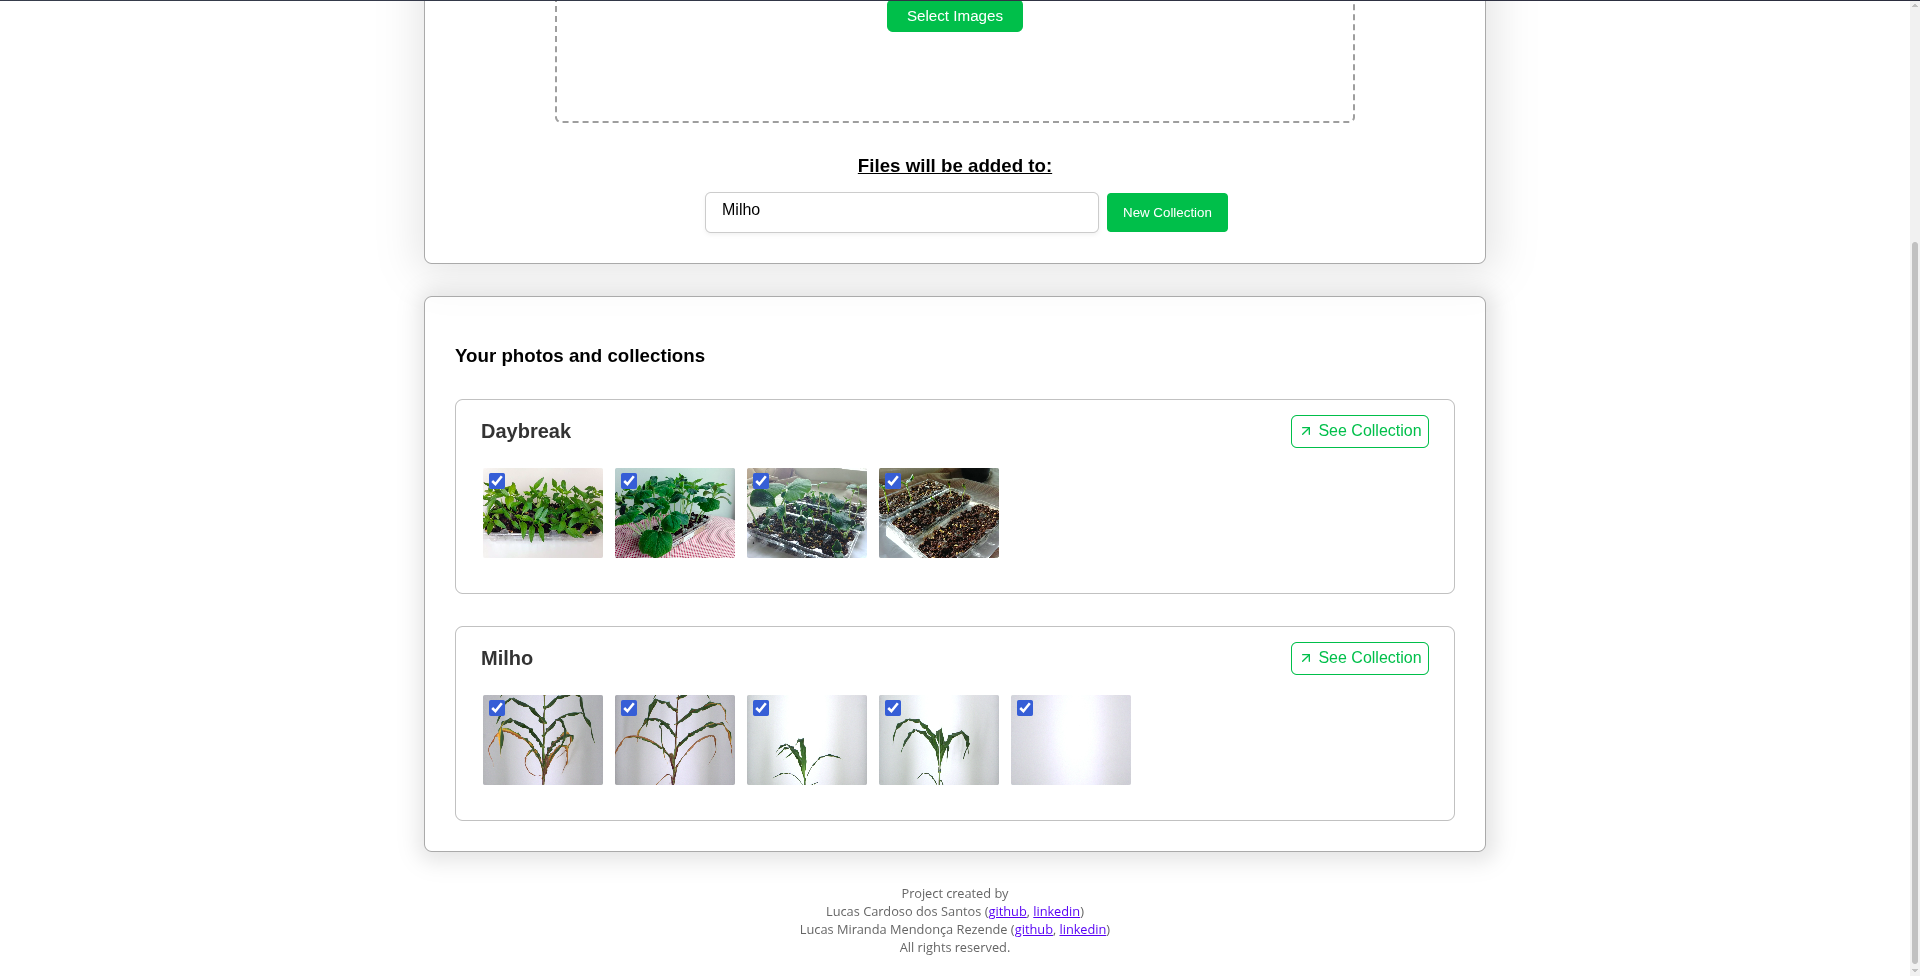
\includegraphics[width=0.9\textwidth]{../figures/screens/colecoes.png}
    \caption{Visualização das coleções de imagens na interface gráfica. Fonte: os autores.}
    \label{fig:colecoes}
\end{figure}

\textbf{2. Visualização dos Resultados de Processamento de uma Imagem:} Ao selecionar uma imagem dentro de uma coleção, o usuário acessa uma tela dedicada à análise individual. Nela, são exibidos lado a lado a foto original e o resultado do processamento: a máscara segmentada sobreposta, as medidas morfológicas extraídas (área, altura e largura) e informações detalhadas sobre a imagem. A Figura~\ref{fig:processamento-individual} mostra um exemplo dessa visualização.

\begin{figure}[H]
    \centering
    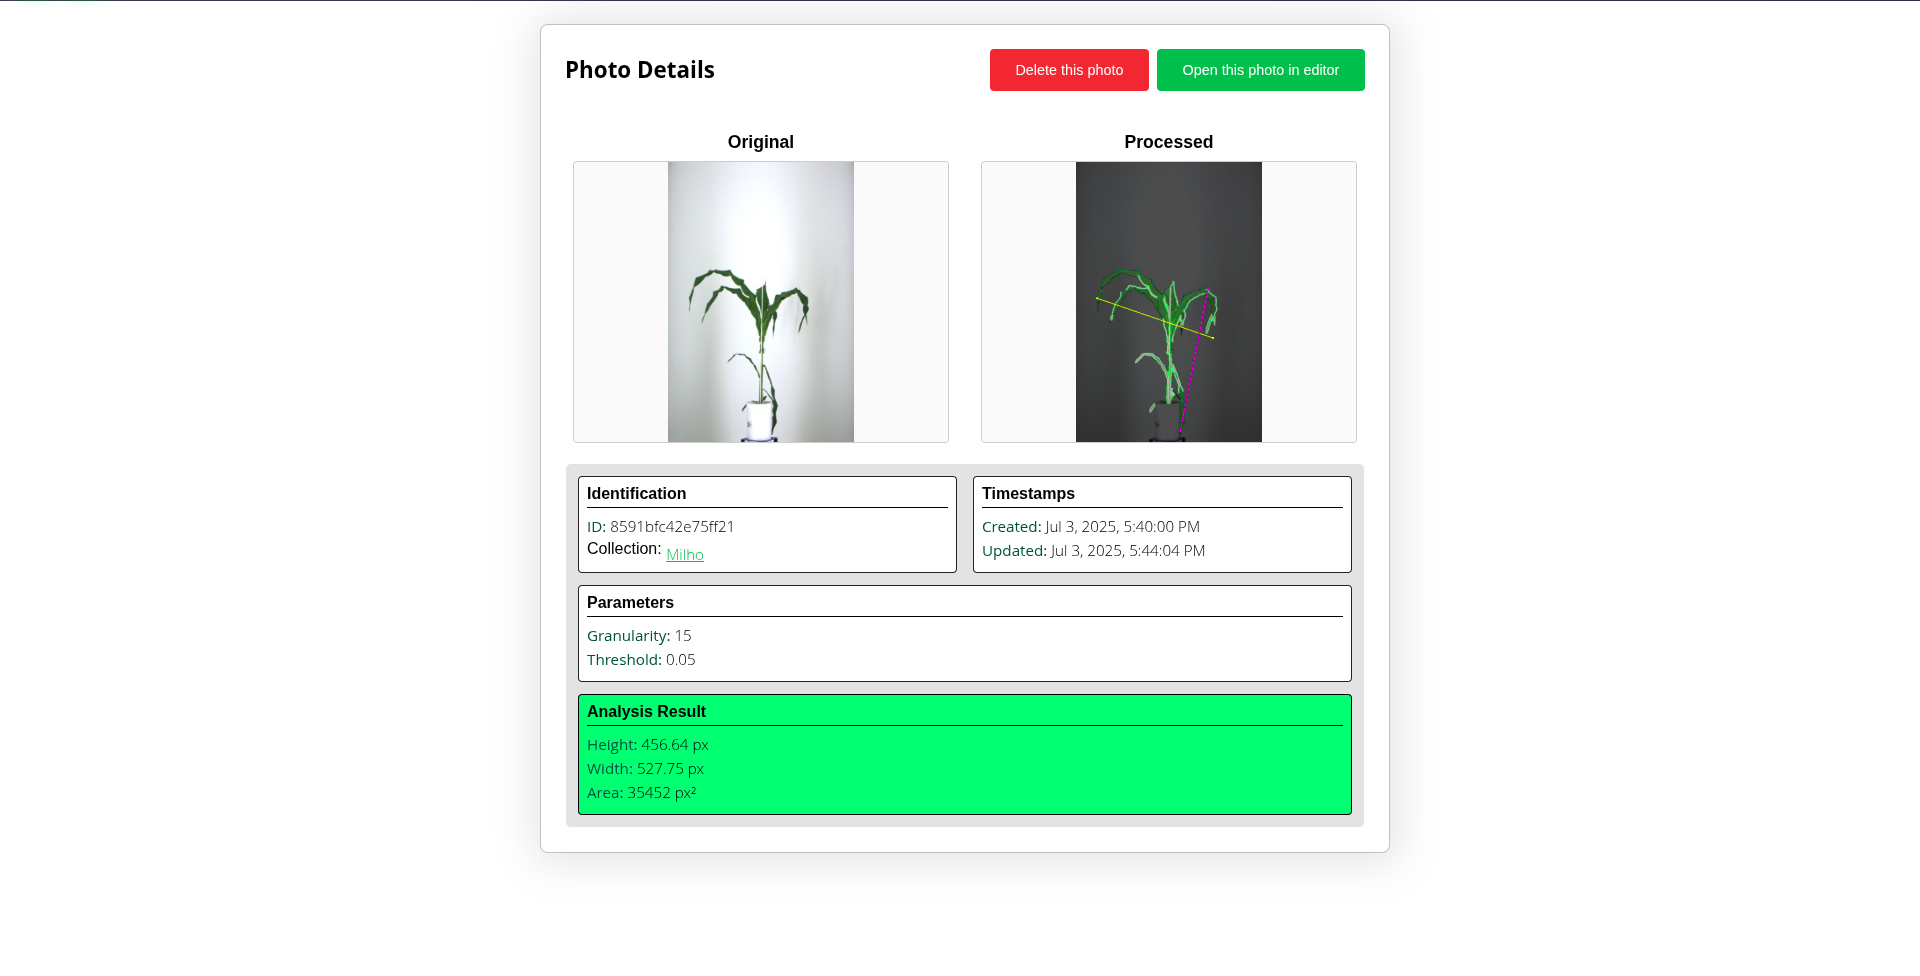
\includegraphics[width=0.9\textwidth]{../figures/screens/processamento-individual.png}
    \caption{Tela de processamento de uma imagem individual, mostrando a visualização dos resultados de segmentação e as medidas extraídas. Fonte: os autores.}
    \label{fig:processamento-individual}
\end{figure}

\textbf{3. Gráficos de Crescimento em uma Coleção:} Para cada coleção, a aplicação gera automaticamente gráficos que mostram a evolução das medidas morfológicas ao longo do tempo, como a área foliar, altura e largura. Esses gráficos permitem ao usuário acompanhar visualmente o desenvolvimento das plantas, identificar tendências e comparar diferentes experimentos. A Figura~\ref{fig:grafico-crescimento} apresenta um exemplo de gráfico de crescimento gerado pela aplicação.

\begin{figure}[H]
    \centering
    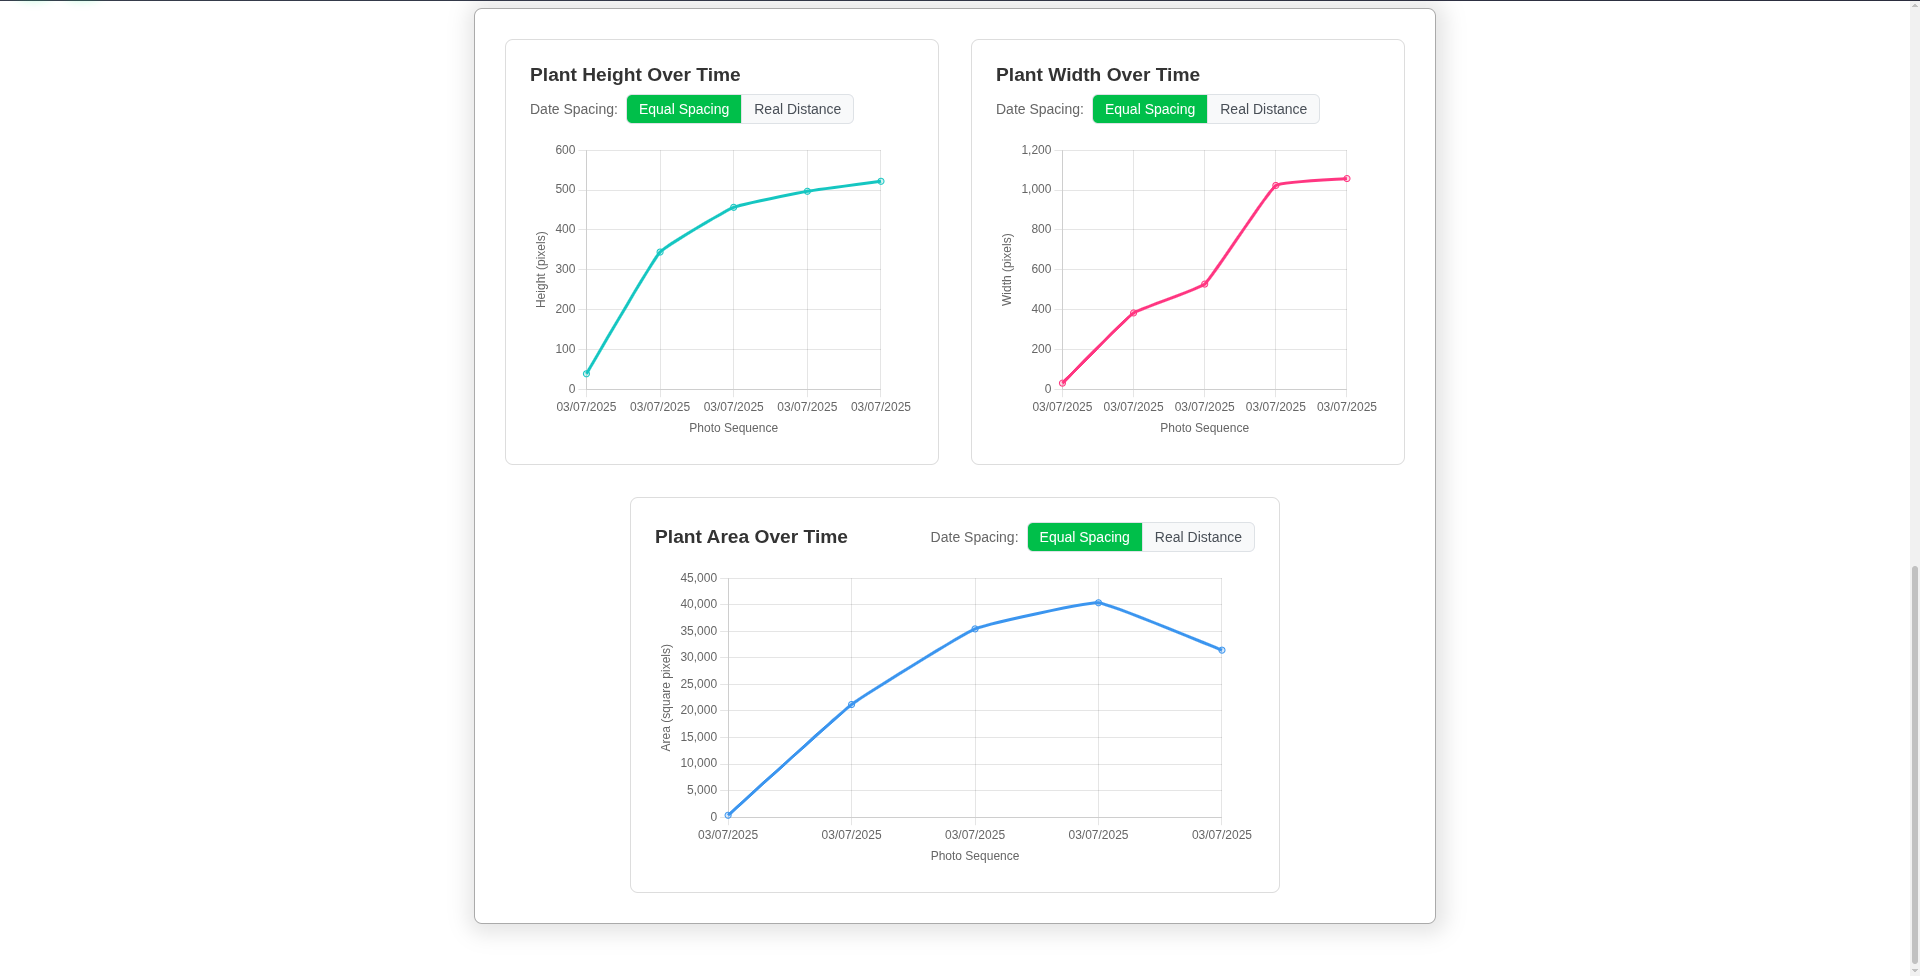
\includegraphics[width=0.9\textwidth]{../figures/screens/grafico-crescimento.png}
    \caption{Gráfico de crescimento mostrando a evolução da área foliar ao longo do tempo em uma coleção. Fonte: os autores.}
    \label{fig:grafico-crescimento}
\end{figure}

Esses resultados demonstram que a solução proposta é eficaz para monitorar o desenvolvimento de plantas de forma automatizada, reprodutível e acessível, atendendo tanto a demandas de pesquisa quanto de ensino ou hobby.


